\section{Mô tả thiết kế kiến trúc để xây dựng hệ thống}
    \quad Sau khi xác định rõ bài toàn, dựa trên những yêu cầu cả về mặt chứng năng và phi chức năng, nhóm quyết định đưa ra thiết kế hệ thống như sau:
    
    \vspace{1cm}
    \begin{figure}[h]
    	\centering
    	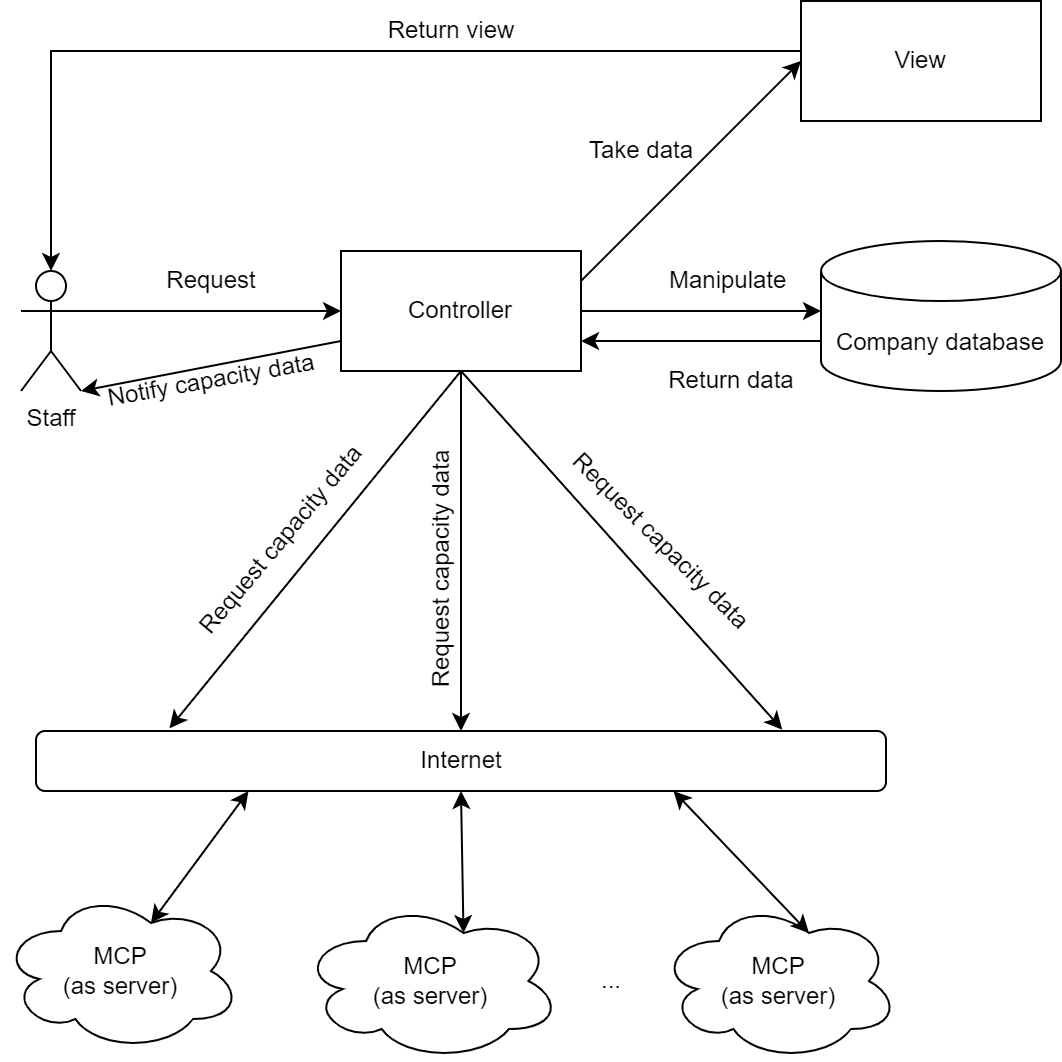
\includegraphics[width=1\linewidth]{imgs/architecture design.png}
    	\caption{Thiết kế kiến trúc của hệ thống}
    \end{figure}
    
    
   	\begin{tblr}{
   			width=1\linewidth,
   			hlines,
   			vlines,
   			colspec={X[3]X[7]},
   			columns = {valign = m, },
   			row{1} = {halign = c, valign = m, bg = lightgray, fg = black},
   		}
   		{\textbf{Table} & \textbf{Architecture design}}  \\
   		Pattern	& MVC + Client-server \\
   		Description & 1. Với các thông tin cơ bản như thông tin cá nhân, lịch làm, thông tin về phương tiện, ta sử dụng mô hình MVC để lấy dữ liệu và hiển thị lên cho người dùng \newline
   		2.Đối với thông tin về sức chứa của các MCPs: coi các MCP như là những server nhỏ, thực hiện chức năng thu thập thông tin về sức chứa do cảm biến ghi nhận. Cứ mỗi 15 phút, controller sẽ request thông tin về sức chứa MCP từ các server   \\
   		Advantages & 1. Thông tin các MCPs sẽ dễ cập nhật, lưu trữ hơn. \newline
   		2. Các sever lưu trữ là riêng biệt nên khi 1 sever của 1 MCP bị sự cố sẽ không ảnh hưởng đến các sever khác. \newline
   		3. Hiển thị dữ liệu theo những cách khác nhau cho các đối tượng \newline
   		4. Dễ mở rộng    \\
   		Disadvantages & 1. Chi phí thiết lập, duy trì các sever trong client-sever khá cao \newline
   		2. Tốc độ phụ thuộc vào tốc độ internet \\
   		Flow & 1. Controller nhận request từ người dùng -> gọi đến database thực hiện yêu cầu -> database gửi kết qua sau khi thực hiện lại cho controller -> controller gửi dữ liệu vừa nhận được cho phần View -> View hiển thị kết quả cho người dùng.newline \newline
   		\newline
   		2. Controller yêu cầu thông tin từ các MCP -> MCP nhận request và trả về thông tin cho Controller -> Controller thông báo thông tin cho người dùngnewline \\
   	\end{tblr}
   
   	\vspace{0.5cm}
   
   	\quad Đối với bài toán được đặt ra, ta sẽ có tổng cộng 6 module. Bao gồm:
   	\begin{enumerate}
   		\item Module Xác thực
   		
   		\begin{tblr}{
   				width=1\linewidth,
   				hlines,
   				vlines,
   				colspec={X[3]X[7]},
   				columns = {valign = m, },
   			}
   			Input & Người dùng X \\
   			Output & Người dùng X có được truy cập hay không \newline
   					 Vai trò của người dùng X là gì \\
   			Method & Validation() \newline
   			 		 Login() \newline
   			 		 Logout() \newline
   			 		 ChangePassword() \\
   		\end{tblr}
   	   		
   		\item Module Chat
   		
  		\begin{tblr}{
  				width=1\linewidth,
  				hlines,
  				vlines,
  				colspec={X[3]X[7]},
  				columns = {valign = m, },
  			}
  			Input & Tin nhắn, văn bản\\
  			Output & Hệ thống gửi tin nhắn cho người dùng \newline
  					 Người dùng nhận được tin nhắn \\
  			Method & ConnectUser() \newline
		  			 SendMessage() \newline
		  			 NotifyMessage() \\
  		\end{tblr}
  	
  		\newpage
  		\item Module View information
  		
  		\begin{tblr}{
  				width=1\linewidth,
  				hlines,
  				vlines,
  				colspec={X[3]X[7]},
  				columns = {valign = m, },
  			}
  			Input & MCP X \newline
  			Phương tiện Y \newline
  			Nhân viên Z \\
  			Output & Thông tin của MCP X \newline
  			Thông tin phương tiện Y \newline
  			Thông tin nhân viên và lịch làm của nhân viên Z \\
  			Method & ShowInfoMCP() \newline
  			ShowInfoVehicle() \newline
  			ShowInfoStaff() \newline
  			ShowDailyTask() \newline
  			ShowCalendar() \\
  		\end{tblr}
   		
   		\item Module Manage Resource
   		
   		\begin{tblr}{
   				width=1\linewidth,
   				hlines,
   				vlines,
   				colspec={X[3]X[7]},
   				columns = {valign = m, },
   			}
   			Input & Nhân viên X, phương tiện Y\\
   			Output & Nhân viên X được chỉnh sửa \newline
   					 Phương tiện Y được chỉnh sửa \\
   			Method & AddUser() \newline
		   		     EditUser() \newline
		   			 DeactivateUser() \newline
   					 \newline
		   			 AddVehicle() \newline
		   			 EditVehicle() \newline
		   			 DeactivateVehicle() \\
   		\end{tblr}
   		
   		\item Module Planning route
   		
   		\begin{tblr}{
   				width=1\linewidth,
   				hlines,
   				vlines,
   				colspec={X[3]X[7]},
   				columns = {valign = m, },
   			}
   			Input & MCP, Vehicle \\
   			Output & Tuyến đường khả dụng \\
   			Method & GenerateRoute() \newline
	   				 PlanRoute() \newline
	   				 GetAvailablePaths() \newline
	   				 ModifyRoute() \newline
	   				 ValidateRoute() \newline
	   				 GetPathsBetween() \newline
	   				 ValidatePath() \\
   		\end{tblr}
   		
   		\newpage
   		\item Module Task assign
   		
   		\begin{tblr}{
   				width=1\linewidth,
   				hlines,
   				vlines,
   				colspec={X[3]X[7]},
   				columns = {valign = m, },
   			}
   			Input &	Nhân viên X \newline
   				    Công việc Y \\
   			Output & Công việc được chia thành công cho nhân viên \newline
   					 Thông báo lịch làm cho nhân viên \\
   			Method & CreateTask() \newline
   					 SetMCP() \newline
   					 SetVehicle() \newline
   					 SetSchedule() \newline
   					 AssignTask() \\
   		\end{tblr}
   		
   	\end{enumerate}
   